
% RECOMMENDED %%%%%%%%%%%%%%%%%%%%%%%%%%%%%%%%%%%%%%%%%%%%%%%%%%%
\documentclass[graybox]{svmult}

% choose options for [] as required from the list
% in the Reference Guide

\usepackage{mathptmx}       % selects Times Roman as basic font
\usepackage{helvet}         % selects Helvetica as sans-serif font
\usepackage{courier}        % selects Courier as typewriter font
\usepackage{type1cm}        % activate if the above 3 fonts are
                            % not available on your system
%
\usepackage{makeidx}         % allows index generation
\usepackage{graphicx}        % standard LaTeX graphics tool
                             % when including figure files
\usepackage{multicol}        % used for the two-column index
\usepackage[bottom]{footmisc}% places footnotes at page bottom

% see the list of further useful packages
% in the Reference Guide

\makeindex             % used for the subject index
                       % please use the style svind.ist with
                       % your makeindex program

%%%%%%%%%%%%%%%%%%%%%%%%%%%%%%%%%%%%%%%%%%%%%%%%%%%%%%%%%%%%%%%%%%%%%%%%%%%%%%%%%%%%%%%%%
\usepackage{multirow}

\begin{document}

\title*{Tumores cerebrais na infância e adolescência}
% Use \titlerunning{Short Title} for an abbreviated version of
% your contribution title if the original one is too long
\author{Francisco Hélder Cavalcante Félix e Juvenia Bezerra Fontenele}
% Use \authorrunning{Short Title} for an abbreviated version of
% your contribution title if the original one is too long
\institute{Francisco Hélder Cavalcante Félix \at Centro Pediátrico do Câncer, Hospital Infantil Albert Sabin, R. Alberto Montezuma, 350, 60410-780, Fortaleza - CE \email{fhcflx@outlook.com}
\and Juvenia Bezerra Fontenele \at Faculdade de Farmácia, Odontologia e Enfermagem, Universidade Federal do Ceará, R. Alexandre Baraúna, 949, 60430-160, Fortaleza - CE %\email{juvenia.fontenele@gmail.com}
}
%
% Use the package "url.sty" to avoid
% problems with special characters
% used in your e-mail or web address
%
\maketitle

\abstract{Os tumores cerebrais são um grupo heterogêneo de doenças neoplásicas de comportamento variável, com as características comuns de relativa raridade, elevada morbidade e elevada mortalidade. Dentre as neoplasias infantis, no entanto, constituem (como um grupo) o primeiro tumor sólido e a segunda neoplasia maligna mais frequente nas crianças, atrás apenas das leucemias, perfazendo em torno de \(20\%\) das neoplasias pediátricas. A sua incidência varia de acordo com a região do mundo. Nos EUA, a incidência anual ajustada para a idade de tumores cerebrais malignos primários na população de \(0-15\) anos foi de \(3,4\) por \(10^5\) pessoas-ano entre \(2004-2008\). Já na Europa, entre \(1988-1997\), a incidência reportada foi de \(2,99\) por \(10^5\). Esta incidência é mais alta do que a usualmente reportada na Ásia, onde relatos indicam entre \(1,8-2,2\) casos por \(10^5\). No Brasil, o primeiro relato do Registro de Câncer de Base Populacional indicou uma incidência de \(0,9\) a \(3,2\) por \(10^5\), semelhante à estatística do mundo desenvolvido ocidental. Hoje em dia, no entanto, já não é apropriado falar em “tumores cerebrais” infantis, sem separar as diversas entidades patológicas entre si, as quais têm incidência, tratamento e prognóstico muito díspares.}

\section{Histórico}
O renomado oncologista Siddharta Mukherjee denominou o câncer de "O Imperador de Todas as Moléstias" (Mukherjee, 2010). Em sua análise histórica, ele mostrou como a humanidade tem se relacionado com o que nós conhecemos modernamente como câncer ao longo de sua história, especialmente no último século, quando começou a organizar-se o campo da oncologia. Os primeiros registros sobre câncer são atribuídos a Imotep (2655-2600 a.C.), o qual viveu a quase 5 mil anos atrás, na terceira dinastia do Egito. No papiro de Edwin Smith (1832-1906), o mais antigo registro escrito relacionado à Imotep, a palavra "cérebro" é mencionada num contexto médico pela primeira vez que se tem notícia (Feldman, 1999). O conceito do câncer como processo patológico deriva das escolas hipocráticas antigas. "Câncer" vem do termo grego carcinos (\(\kappa \alpha \rho \kappa \iota \nu o \zeta\), "karkinos") , o qual significa "caranguejo" e era usado na medicina correspondendo a vários tipos de lesões tumorais e úlceras crônicas (Goodrich, 2013). O enciclopedista médico Celso (25 a.C.-50 d.C.) traduziu carcinos como cancer e cunhou o termo carcinoma (Celso, 1753). 

Galeno (130-200) introduziu o termo oncos como referência ao estudo dos tumores e criou a teoria humoral, popular por muitos séculos depois dele (Galeno, 1854-1856). Na baixa idade média, a medicina foi dominada pelos autores árabes e o Cânone de Avicena (980-1037) tinha detalhadas descrições sobre o comportamento dos tumores malignos, incluindo sua invasividade local, destruição tecidual, perda de funções afetadas e, finalmente, disseminação distante com a morte como consequência (Avicena, 1973). Durante todo este longo período, não existe menção à cirurgia como tratamento de tumores cerebrais. O tratamento clínico, por sua vez, seguia as recomendações da teoria humoral de Galeno, com purgativos e sangria. Antes disso, na antiguidade clássica, as escolas hipocráticas usavam medicina herbária para mitigar os sintomas e trazer conforto para os pacientes. Nenhuma mudança significativa ocorreu até a Renascença, quando o conhecimento anatômico e a fisiologia começaram a ser revolucionados. 

Não antes dos séculos 18 e 19, surgiram descrições mais precisas acerca de tumores cerebrais. A partir deste período, com o desenvolvimento cada vez maior da cirurgia, com o advento da antissepsia e da anestesia e com os progressos da patologia, o conceito de câncer e seu tratamento como nós o conhecemos hoje surgiu (Goodrich, 2013). Com o advento do conhecimento sobre a localização de funções e lesões neurológicas, neurologistas como Gowers (1845-1915) puderam guiar cirurgiões como Horsley (1857-1916) a realizar as primeiras cirurgias neurooncológicas bem sucedidas, inaugurando o que se tornaria, no século 20, a moderna neurooncologia (Gowers, 1888). Digno de nota é o fato de que uma das primeiras neurocirurgias bem sucedidas para a retirada de um tumor intracraniano ocorreu em 1879 e a paciente era uma menina de 14 anos, portadora de um meningioma (Macewen, 1888).

\section{Tumores cerebrais pediátricos}
\label{sec:1}
Os tumores cerebrais são um grupo heterogêneo de doenças neoplásicas de comportamento variável, com as características comuns de relativa raridade, elevada morbidade e elevada mortalidade. Dentre as neoplasias infantis, no entanto, constituem (como um grupo) o primeiro tumor sólido e a segunda neoplasia maligna mais frequente nas crianças, atrás apenas das leucemias, perfazendo em torno de \(20\%\) das neoplasias pediátricas. A sua incidência varia de acordo com a região do mundo. Nos EUA, a incidência anual ajustada para a idade de tumores cerebrais malignos primários na população de \(0-15\) anos foi de \(3,4\) por \(10^5\) pessoas-ano entre \(2004-2008\) \cite{Ostrom01102014}. Já na Europa, entre \(1988-1997\), a incidência reportada foi de \(2,99\) por \(10^5\) \cite{Peris-Bonet}. Esta incidência é mais alta do que a usualmente reportada na Ásia, onde relatos indicam entre \(1,8-2,2\) casos por \(10^5\) \cite{CNCR21430}. No Brasil, o primeiro relato do Registro de Câncer de Base Populacional indicou uma incidência de \(0,9\) a \(3,2\) por \(10^5\), semelhante à estatística do mundo desenvolvido ocidental \cite{IJC24799}. Fortaleza teve uma das menores incidências relatadas, \(1,3\) casos por \(10^5\), o que pode indicar subdiagnóstico. Hoje em dia, no entanto, já não é apropriado falar em “tumores cerebrais” infantis, sem separar as diversas entidades patológicas entre si, as quais têm incidência, tratamento e prognóstico muito díspares.

Os tumores cerebrais mais frequentes em crianças são os astrocitomas pilocíticos, tumores de comportamento incerto, ora classificados como benignos, ora como malignos. Eles representam em torno de 1\(8\%\) dos tumores cerebrais infantis. Em seguida, vem os tumores embrionários, a maior parte dos quais meduloblastomas, os tumores malignos mais comuns da infància, que representam em torno de \(15\%\) dos diagnósticos de tumor cerebral em crianças \cite{Ostrom01102014}. Astrocitomas pilocíticos são tumores indolentes, de crescimento lento, tratados principalmente pela ressecção cirúrgica, a qual é curativa na maioria dos casos, com pouca probabilidade de disseminação e virtualmente ausência de transformação maligna \cite{gan}. Já os meduloblastomas são tumores indiferenciados, com elevado índice mitótico, com acentuada propensão à disseminação e recidiva, necessitando de terapia adjuvante com radioquimioterapia após ressecção cirúrgica \cite{partap}. Estes dois tipos tumorais, que juntos correspondem a mais de \(30\%\) dos casos de tumores cerebrais em crianças, têm hoje um excelente prognóstico quando comparado ao passado. Outros tipos tumorais menos frequentes, todavia, têm resultados menos brilhantes com o tratamento atualmente disponível. Tumores de tronco cerebral, normalmente não biopsiados na sua maioria, constituem cerca de \(10\%\) dos tumores cerebrais infantis, e têm um prognóstico extremamente reservado, com apenas um subgrupo pequeno de pacientes com tumores neste sítio alcançando sobrevida prolongada.

O tratamento de tumores cerebrais em crianças e adolescentes evoluiu significantemente nas últimas décadas. Dos anos 80 até hoje, o conhecimento sobre o papel das várias modalidades de terapia (cirurgia, radioterapia e quimioterapia) ficou mais claro e programas terapêuticos específicos para cada tipo de doença puderam ser desenvolvidos. Hoje em dia, a maioria das crianças com um diagnóstico de tumor cerebral conseguirá ser adequadamente tratada e alcançará sobrevida prolongada. O manejo dos efeitos colaterais a longo prazo da terapia e das sequelas da doença são as principais preocupações na neuro-oncologia pediátrica moderna \cite{merchant}. No Brasil, estudos de sobrevida de pacientes pediátricos com tumores cerebrais são raros. Nosso grupo publicou recentemente uma análise de sobrevida de \(103\) pacientes pediátricos diagnosticados com tumores cerebrais entre 2000 e 2006 num único centro hospitalar, mostrando resultados que se assemelham aqueles dos registros populacionais dos EUA e Europa para as principais patologias \cite{araujo}.

\begin{center}
\begin{table}
\renewcommand{\arraystretch}{1.5}
	\caption{\small incidência relativa de grupos histológicos de tumores cerebrais em criança e adolescentes relatada no Brasil. A classificação está de acordo com a Classificação Internacional do Câncer na Infância (CICI), terceira edição \cite{CNCR20910}. A última coluna mostra dados não publicados de nosso serviço. P = Pinho et al, 2011 \cite{pinho}; R = Rosemberg et al, 2007 \cite{ros}; H = HIAS, não publicado; NI = não informado; PNET = \textit{primitive neuroectodermal tumor} (tumor neuroectodérmico primitivo); DNET = \textit{Dysembryoplastic neuroepithelial tumor} (tumor neuroepitelial disembrioplásico); DIG/A = \textit{Desmoplastic infantile ganglioglioma/ astrocytoma} (ganglioglioma/ astrocitoma infantil desmosplásico).}
\begin{tabular}{c|c|ccc|c|c}
	\hline
	\multicolumn{4}{c|}{Tipos tumorais (histologia)}&{P}&{R}&{H}	\\
	\hline
	\multicolumn{1}{c|}{\multirow{15}{*}{Neuroepiteliais}}&{\multirow{7}{*}{Gliomas}}&{\multirow{3}{*}{Astrocitomas}}&\multicolumn{1}{|c|}{Pilocítico}&{\multirow{3}{*}{37\%}}&{18,2\%}&{10,6\%}
	\\
	\cline{4-4}\cline{6-7}
    \multicolumn{1}{c|}{}&&&\multicolumn{1}{|c|}{Difuso}&&{6,2\%}&{7\%}\\
	\cline{4-4}\cline{6-7}
    \multicolumn{1}{c|}{}&&&\multicolumn{1}{|c|}{Anaplásico}&&{4,4\%}&{2,2\%}\\
	\cline{3-7}
    \multicolumn{1}{c|}{}&{}&\multicolumn{2}{c|}{Oligodendrogliomas}&{NI}&{0,9\%}&{0,9\%}\\
	\cline{3-7}
    \multicolumn{1}{c|}{}&&{\multirow{2}{*}{Ependimomas}}&\multicolumn{1}{|c|}{Clássico}&{\multirow{2}{*}{6,8\%}}&{\multirow{2}{*}{7,4\%}}&{7,9\%}\\
    \cline{4-4}\cline{7-7}
    \multicolumn{1}{c|}{}&&&\multicolumn{1}{|c|}{Anaplásico}&&&{4\%}\\
	\cline{3-7}
    \multicolumn{1}{c|}{}&&\multicolumn{2}{c|}{Glioblastoma}&{NI}&{3,7\%}&{3,5\%}\\
    \cline{2-7}
    \multicolumn{1}{c|}{}&{\multirow{6}{*}{Embrionários}}&{\multirow{3}{*}{Meduloblastomas}}&\multicolumn{1}{|c|}{Clássico}&{\multirow{3}{*}{13,6\%}}&{\multirow{3}{*}{11,2\%}}&{21\%}\\
	\cline{4-4}\cline{7-7}
    \multicolumn{1}{c|}{}&&&\multicolumn{1}{|c|}{Desmoplásico}&&&{3,5\%}\\
	\cline{4-4}\cline{7-7}
    \multicolumn{1}{c|}{}&&&\multicolumn{1}{|c|}{Anaplásico}&&&{0,4\%}\\
	\cline{3-7}
    \multicolumn{1}{c|}{}&{}&\multicolumn{2}{c|}{Pineoblastoma}&{\multirow{3}{*}{3,9\%}}&{NI}&{0,4\%}\\
	\cline{3-4}\cline{6-7}
    \multicolumn{1}{c|}{}&&{\multirow{2}{*}{PNET}}&\multicolumn{1}{|c|}{Supratentorial}&&{\multirow{2}{*}{2,7\%}}&{1,3\%}\\
    \cline{4-4}\cline{7-7}
    \multicolumn{1}{c|}{}&&&\multicolumn{1}{|c|}{Outros}&&&{0,9\%}\\
    \cline{2-7}
    \multicolumn{1}{c|}{}&{\multirow{2}{*}{Neurais e Glioneurais}}&\multicolumn{2}{c|}{Ganglioglioma}&{\multirow{2}{*}{NI}}&{4,6\%}&{0,8\%}\\
    \cline{3-4}\cline{6-7}
    \multicolumn{1}{c|}{}&&\multicolumn{2}{c|}{Neurocitoma, DNET, DIG/A}&&{3\%}&{0\%}\\
    \hline
	\multicolumn{1}{c|}{Meninges}&\multicolumn{3}{c|}{Meningiomas}&{NI}&{3\%}&{NI}\\
	\hline
	\multicolumn{1}{c|}{Endócrino}&\multicolumn{3}{c|}{Craniofaringiomas}&{10,5\%}&{11\%}&{NI}\\
	\hline
	\multicolumn{1}{c|}{TCG}&\multicolumn{3}{c|}{Tumores de células germinativas}&{6,1}&{3,6\%}&{NI}\\
    \hline
\end{tabular}
\end{table}
\end{center}

\begin{center}
\begin{figure}[htpb]
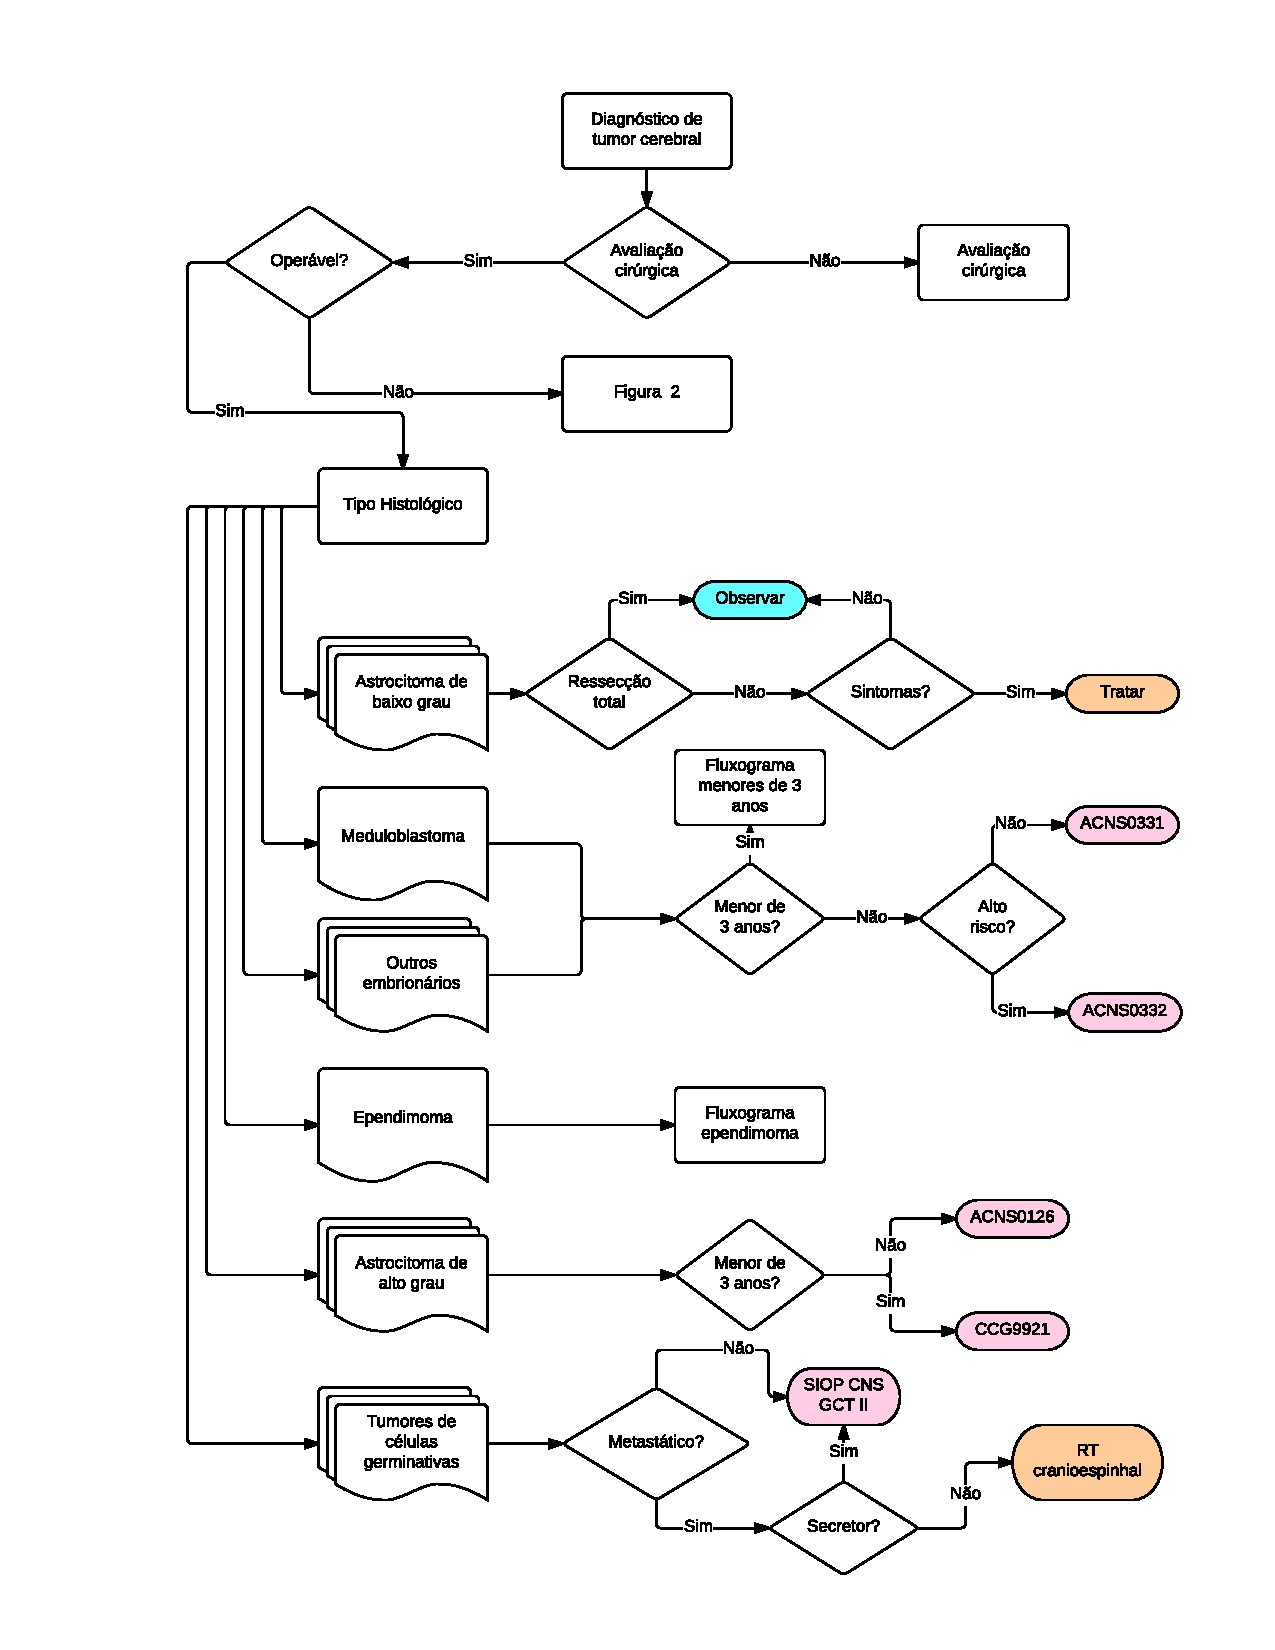
\includegraphics[scale=0.6,trim = 10mm 10mm 11mm 5mm,clip]{fig/fig1.pdf}
\caption{Tratamento de crianças com tumores cerebrais, com histologia}
%\label{Rotulo}
\end{figure}
\clearpage
\begin{figure}[!htb]
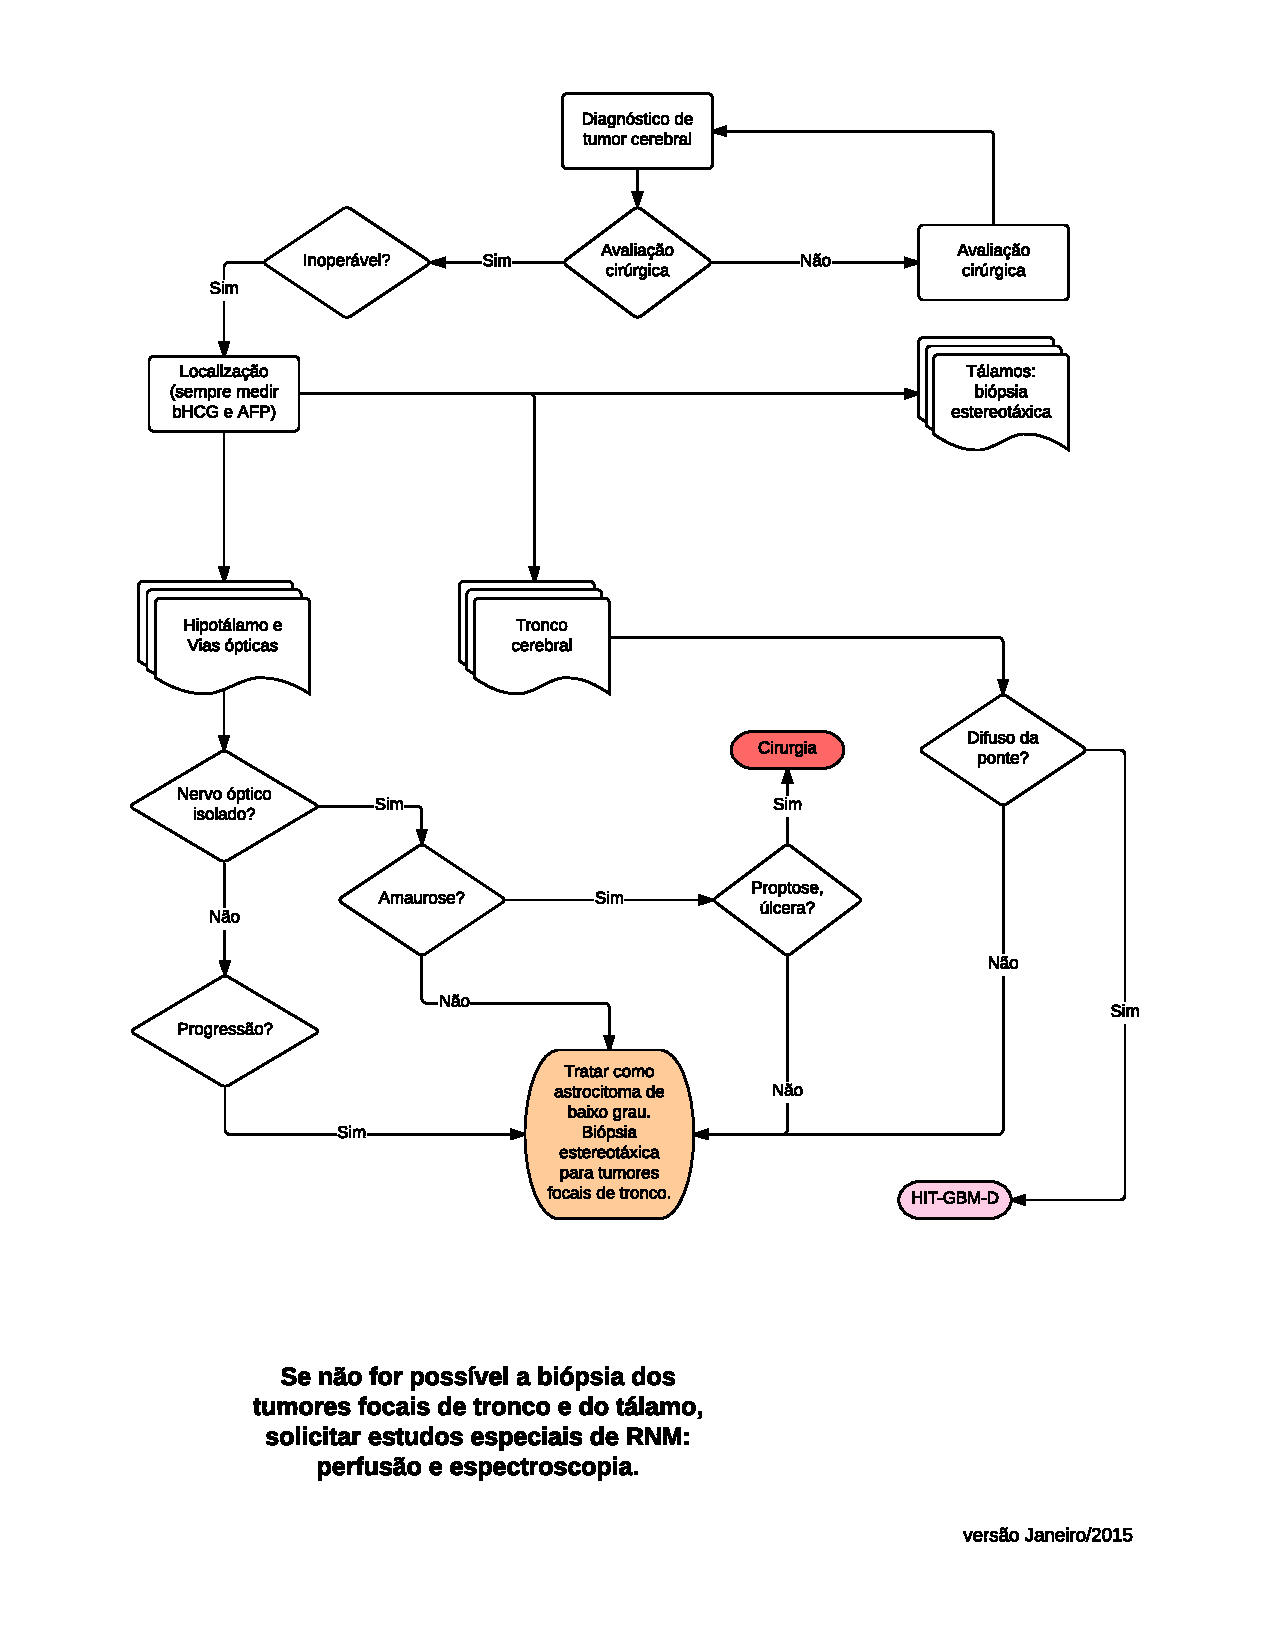
\includegraphics[scale=0.63,trim = 20mm 5mm 10mm 8mm,clip]{fig/fig2.pdf}
\caption{Tratamento de crianças com tumores cerebrais, sem histologia}
%\label{Rotulo}
\end{figure}
\end{center}

\section{Qual o objetivo desta obra}
\label{sec:2}
O Hospital Infantil Albert Sabin (HIAS) é uma instituição da administração direta da Secretaria de Saúde do Estado do Ceará, habilitado como unidade de assistência de alta complexidade em neurologia e neurocirurgia, UNACON exclusiva de oncologia pediátrica, UTI pediátrica nível II e hospital de ensino, nível de atenção de alta complexidade, atendendo pelo SUS \cite{cnes}. O Centro Pediátrico do Câncer é o anexo do HIAS que abriga o tratamento oncológico clínico, contando com equipe multiprofissional de atenção às crianças com câncer. Tem \(22\) leitos de internação em enfermaria (\(2\) isolamentos), \(06\) leitos de UTIP, e \(05\) consultórios para atendimento ambulatorial. O ambulatório e a enfermaria têm material para atendimento às urgências e emergências, incluindo carrinho de emergência completo com drogas e equipamento para reanimação. A enfermaria do CPC conta com plantão médico 24h por dia.

O HIAS-CPC é referência estadual para o tratamento de crianças com tumores cerebrais, servindo uma população de 8,8 milhões de habitantes (um e meio milhão de crianças e jovens até 18 anos) \cite{estat}. A incidência ajustada para a idade de tumores cerebrais pediátricos no Ceará foi estimada em \(1,3\) casos por \(10^5\), entre 1998 e 2002 \cite{inca}. Seu papel é fundamental para o diagnóstico, tratamento e acompanhamento de centenas de crianças com câncer, incluindo tumores cerebrais. O HIAS-CPC recebeu cerca de \(35\) novos pacientes com tumores cerebrais ao ano entre 2007 e 2013 (um total de \(250\)). Isto indica que a esmagadora maioria das crianças com esta doença no estado do Ceará são tratadas no HIAS-CPC. Dessa forma, torna-se imprescindível que a qualidade da atenção à saúde dispensada a estes pequenos pacientes em nosso serviço hospitalar seja continuamente revisada, avaliada e padronizada.

\subsection{Revisão da literatura}
\label{subsec:2}
Os autores utilizaram uma estratégia de busca de mapeamento (mapping review) a fim de estabeler o panorama do conhecimento atual sobre o tratamento de tumores cerebrais em crianças (revisão da literatura, revisão narrativa) \cite{grant,vosgerau}. Uma busca foi realizada no PubMed com os termos “low grade glioma”, “medulloblastoma”, “high-grade glioma”, “brainstem tumor”, “combined treatment” e os filtros “all children” e "clinical trial” (busca original: \texttt{http://bit.ly/fhcflx-2DIR}). O número total de entradas conseguidas com esta estratégia foi de 271 publicações. Uma atualização da busca foi realizada, com o acréscimo de mais 41 trabalhos (\texttt{http://bit.ly/fhcflx-2pnA}). Foram excluídas aquelas sobre adultos ou outras patologias fora do interesse da revisão e também aqueles com mais de 2 décadas e incluídos preferencialmente os ensaios clínicos fase 1, 2 e 3 e as revisões sistemáticas. A bibliografia dos trabalhos selecionados foi checada para identificar trabalhos dentro do escopo do projeto. Os trabalhos incluídos no final são os citados na bibliografia da revisão, nesta obra. Os trabalhos foram revisados e qualificados segundo a nova classificação de níveis de evidência da OCEBM \cite{ocebm}. De acordo com a classificação 2011 da OCEBM, os ensaios controlados e randomizados são considerados evidência de nível 2, enquanto os estudos não controlados e séries de casos (equivalentes) são considerados evidência de nível 4 (tratamento). Nenhum trabalho com nível 3 de evidência (controlados, porém não randomizados) foi encontrado. Alguns ensaios foram desenhados para obter informações sobre história natural da doença. Grandes coortes para estudo de prognóstico (\textit{inception cohort}) são consideradas nível 2 de evidência, enquanto coortes de qualidade menor ou grupos controle de ensaios randomizados são nível 3.

A partir deste mapeamento, foram selecionados os tratamentos com maior qualidade de evidência. Lacunas no conhecimento atual foram listadas (não exaustivamente). Esta evidência foi usada para esboçar um plano ótimo de tratamento para os pacientes. As dúvidas em relação a indicação de modalidades específicas de tratamento foram discutidas e possíveis implementações práticas foram sugeridas. O resultado é um texto cujo objetivo é esclarecer quais as opções de tratamento disponíveis, quais são amplamente aceitas como padrão, onde existe controvérsia e onde a evidência está faltando para indicar um determinado tratamento. O intuito não é ser uma diretriz ou protocolo (vide definições), mas embasar a análise crítica dos protocolos utilizados no serviço do Hospital Infantil Albert Sabin (HIAS), para o tratamento de crianças e adolescentes portadores de tumores cerebrais.

\subsubsection{Protocolos de tratamento utilizados no HIAS}
Na segunda parte desta obra, os protocolos utilizados para tratar os pacientes com tumores do sistema nervoso central no HIAS foram listados e apresentados. Avaliamos todos os protocolos de tratamento utilizados no nosso serviço hospitalar para tratar crianças e adolescentes com tumores do sistema nervoso central, atraveés de revisão de prontuários. O período avaliado foi os últimos 16 anos. Um total de 262 pacientes foram tratados com quimioterapia antineoplásica citotóxica sistêmica nesse período. Destes, 105 (40\%) estavam vivos até a última atualização desta obra. Os protocolos de tratamento clínico usados em nosso serviço foram: COG-A9952 \cite{Ater20072012} (107 pacientes), SOBOPE 1998 (52 pacientes), HIT-GBM-C ou D \cite{Wolff2011} (22 pacientes), SLAOP 1993 \cite{slaop1} (21 pacientes), ACNS-0126 \cite{noq191} ou DUMC-1703 (16 pacientes), SIOP CNS GCT I ou II (14 pacientes), CCG-9961 \cite{4980} (10 pacientes), CCG-9921 \cite{095} (6 pacientes), COG-A99701 \cite{2792} (6 pacientes), outros (5 pacientes). 

Nos anexos desta obra, colocamos as fichas de tratamento que são usadas nos prontuários dos pacientes com tumores do sistema nervoso central tratados no HIAS. O tratamento apenas inicia depois que os pais ou responsáveis legais são informados sobre a proposta de tratamento e as opções disponíveis. Dividimos os anexos de acordo com o tipo de tratamento proposto para os pacientes: quimioterapia de primeira linha (protocolos usados via de regra como primeira escolha no tratamento, baseados na melhor evidência disponível modernamente), quimioterapia de resgate (usados para tratar doenças recorrentes, muitas vezes baseados em evidência mais limitada), quimioterapia neoadjuvante (realizada antes do tratamento cirúrgico definitivo) e quimioterapia metronômica (tem efeito anti-angiogênico e um esquema de doses pequenas e frequentes, em geral paliativo). Além disso, acrescentamos mais 3 seções para protocolos alternativos (substituídos por novos esquemas ou abandonados), terapia biológica, imunoterapia e terapia-alvo (usando anticorpos monoclonais, inibidores de tirosina quinase ou drogas imunomoduladoras), e protocolos experimentais (não usados na rotina de tratamento dos pacientes, apenas ensaios clínicos).

No capítulo sobre os protocolos usados no HIAS, fornecemos maiores detalhes sobre como foram elaborados e como são usados no nosso serviço.

\bibliographystyle{unsrt}
\bibliography{cpc-neuro2014/bib}

\end{document}
